\documentclass{article}
\usepackage[utf8]{inputenc}
\usepackage{graphicx}
\graphicspath{ {images/} }

\usepackage{biblatex}
\addbibresource{main.bib}

\title{PeaCrow: Automated Goal Resolution in Coq}
\author{Ben Jones, Julie L. Newcomb, Daryl Zuniga}
\date{June 3, 2016}

\begin{document}

\maketitle

\section{Introduction}
While automated theorem provers have made enormous strides in recent years, most large, real-world software verification projects are done in proof assistants. Even for experienced proof engineers, completing proofs is a difficult task that requires the user to stop and think often. During a session with a proof assistant, the user’s CPU is idle while the proof assistant is waiting for the next command from the user. This is wasteful; having the CPU do literally anything useful while waiting for user input would be an improvement. We have built PeaCrow, a tool to enhance proof development in Coq that uses those spare cycles to do proof synthesis in the background to aid the user, without interfering with the user’s current workflow.

\section{Overview and Related Work}
PeaCoq is a browser-based front end UI for the Coq proof assistant developed by Valentin Robert and Sorin Lerner at UC San Diego.\cite{peacoq} It provides similar views of goals and hypotheses that most proof editors do, and in addition allows previewing the results of running a tactic on the current proof state without losing the current proof state. It is implemented as a Haskell server which can interface directly with Coq; this server will try a tactic and report the result, but then undo the tactic in the running Coq instance, so that the state of the proof includes only tactics that the user has written. The results are passed to a Javascript frontend and displayed to the user.

We built off of this Javascript frontend to implement autocomplete for proofs in PeaCoq. Based on the current proof state, we synthesize potential proof scripts for each current goal and then send them to Coq to validate. If a generated proof is verified as correct, we notify the user and then attempt to find a simpler version of that proof. As soon as the user is notified of a proof completion, they may insert it into their current proof through a menu selection or a keyboard shortcut. A key design principle in this system was to avoid ever interrupting the user either visually or via resource starvation. By building this capability into PeaCoq, we have brought some of automated theorem proving into an otherwise manual process.

Merging manual and automated theorem proving is not a new idea. By far the most successful implementation is the Sledgehammer subsystem of the Isabelle/HOL proof system. Isabelle/HOL is similar to Coq in that it is a proof-plan based proof assistant. Rather that write inference rules directly in the underlying logic, Isabelle users write in a tactics meta-language called Isar \cite{dennis2006comparison}. The Sledgehammer translates proof goals into a common higher-order-logic format that many automated theorem provers use as input, and selects a heuristically determined set of contextual information. This is then sent to a suite of up to 17  automated theorem provers that are run in parallel \cite{blanchette2011hammering}. Whenever one of them reports a proof is found, Sledgehammer attempts to translate that proof back into Isar, and if it is successful offers the proof to the user \cite{meng2006automation}.

No such system previously existed for Coq. Additionally Sledgehammer has different design considerations than PeaCrow. Sledgehammer is a very heavyweight tool, often taking several minutes to return a result. As such, it is not run automatically, but is rather invoked by the user. This has lead to a common workflow of users preferring to lay out a proof and run sledgehammer on individual parts sequentially, walking away during each invocation rather than continuing to build the proof themselves. If the Sledgehammer does not work, then the user may try breaking down the proof statement into a smaller statement. This workflow is common enough that it is now being taught in introductory proof courses that use Isabelle \cite{paulson2010three}.

In contrast, PeaCrow is a fast and lightweight system. We do not do any translation outside of Coq’s tactic meta-language (LTAC), and our tool gets results in seconds, not minutes. This allows PeaCrow to always be running automatically in the background, providing an experience more akin to code completion. It is our hope that these features will make PeaCrow a tool that naturally fits into existing Coq proof workflows.
\section{Algorithm and Encodings}
\begin{figure}
\centering
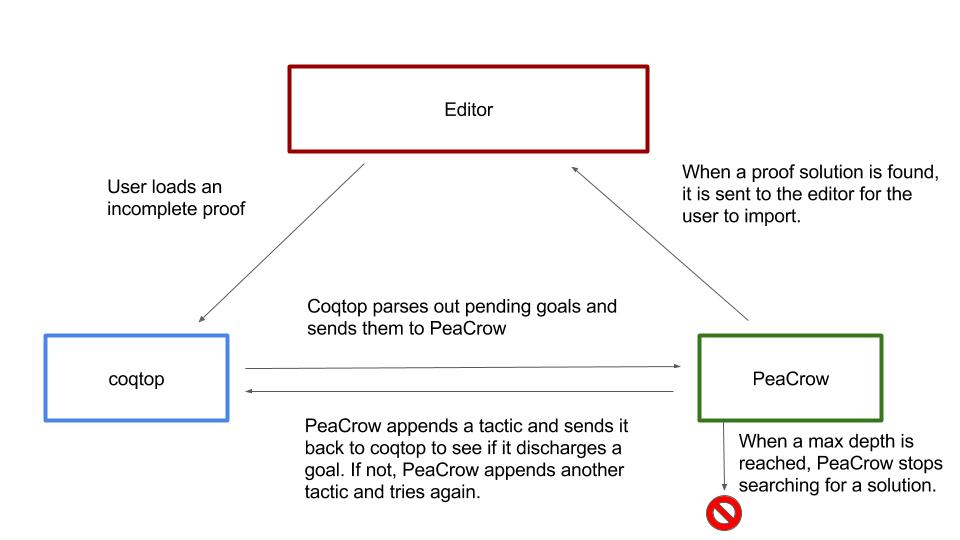
\includegraphics[width=\textwidth]{PeaCrowprocess}
\caption{The process by which PeaCrow searches for a sequence of tactics that can resolve a pending goal.}
\end{figure}
Our approach is to use enumerative synthesis to try to find useful proofs for the user, similar to the SyGuS technique \cite{alur2015syntax}. Much as PeaCoq does, we use coqtop as an oracle to check that our proposed proof completions (1) are valid and (2) will discharge a pending proof goal. The space of all possible proofs is intractably large, containing a large number of possible tactics and an even larger number of lemmas in the Coq standard libraries that can be used as tactic arguments. Since there are few syntactic restrictions on how tactics can follow one another, exploring this space would result in severe path explosion. Instead, we limit ourselves to completing proof goals using a set of non-destructive proof techniques.

Non-destructive proof techniques are a set of tactics we have defined that can only add information to the proof context, never take any away. Essentially they represent forward reasoning. It is always safe to apply one of these tactics to a proof in progress, although we cannot guarantee that they will take us any closer to a goal state. Therefore, we will never need to backtrack after appending a non-destructive tactic. We also defined a set of terminator tactics that, if they succeed, will finish off a goal. For each goal, we first try to discharge it with a terminator tactic. If they all fail, we try appending a non-destructive tactic and try the terminator tactics again. We continue adding non-destructive tactics until a specified bound is reached, at which point the search stops. Using this technique, we only need to maintain a single partial solution per active goal.

Of course, proof completions found in this process may be longer than necessary, since some of the non-destructive tactics may not contribute anything to solving the goal. After a solution to a goal is found, our tool tries to drop as many of its tactics as it can to produce a shorter sequence of tactics that will still discharge the goal. If a minimized solution is found, it is suggested to the user in place of the original solution (note that the solution is ‘minimal’ not with respect to all possible solutions, but for all solutions composed only of our chosen non-destructive and terminator tactics).

One challenge with this approach is that it is important to ensure that non-destructive tactics add non-trivial information to the context. For PeaCrow, we ensure this by disallowing non-destructive tactics from adding hypothesis that are just duplicates of existing hypothesis.
\section{Results}
We added a Goals tab to the PeaCoq editor to supply the results of our proof search to the user. The user can click this tab to see all goals listed; if a solution to a goal has been found, it will also be shown, along with an indicator if it has been found to be minimal. The user can click on the solution to have it appear in their editor window. Also, when the editor pane is focused, the user can press ctrl-space to see any available synthesized solutions appear as an autocomplete suggestion.

One of our main design goals was that PeaCrow should never interfere with the user’s own work. Although the proof synthesis process is continually querying coqtop, if the user advances the cursor over their own proof, they should not notice any slowdown or lag. We solved this problem by maintaining two queues of queries to send to coqtop: those originating from the user and those originating from our synthesis process or PeaCoq’s proof tree process. Synthesis queries are only dispatched to coqtop if all user-originating queries have been addressed. We also took care to keep all goals and solutions available to the user interface in sync with the current state of the proof. If the user makes any change to the proof that made any previous goals obsolete, we invalidate them and remove them from the user interface.

One challenge we faced was in setting up our development environments. Coq is notoriously finicky and has recently undergone a non-backwards compatible version change. The coqtop utility has a mode in which it can be queried by an IDE, but it is barely documented and difficult to set up. For this reason, we wanted to make use of the PeaCoq Haskell server that has already implemented an API for coqtop queries. However, PeaCoq is a work in progress and we were not able to build the most recent version (encountering several different problems on our different platforms). After a long period of experimentation (and many questions to the PeaCoq authors) we were able to build to an older branch of the PeaCoq source code. Unfortunately, that meant we were restricted to an older version of the Javascript-based editor as well (it has since been completely rewritten in Typescript). However, being able to augment an existing editor with our functionality rather than implementing an editor ourselves saved us an enormous amount of work.

\begin{figure}
\centering
\includegraphics[width=\textwidth]{flow}
\caption{PeaCrow Workflow. (1) The user has started a proof. The red Goals badge in the top right indicates that PeaCrow has identified two goals that can be automatically resolved in the current context. The user can either click the badge to view and select these proofs (2a), or press Ctrl-Space to bring up an in-line autocomplete pop-up (2b). In both of these screenshots the Goals badge has turned blue, meaning that PeaCrow has minimized the proofs of all goals. Once the user has selected a goal to complete, it is inserted into the proof buffer and the proof cursor is advanced (3). PeaCrow indicates that there is still one more resolvable goal (4). The user selects this via the autocomplete menu, and the proof is completed (5).}
\end{figure}


Despite these challenges, once we had our tool up and running, we felt that it has real potential. Our “first do no harm” approach means there is no real cost to using our tool, and we can see using it to write proofs as it is. For future work, there are a lot of things we could try to make the synthesis engine more powerful. The first major thing to try would be backtracking search over a wider set of tactics, including destructive ones. In our current search we only have to keep track of one “head” per goal, but in a breadth-first exploration of a large search space we will potentially have to keep track of hundreds or more. We need to make sure that this intensive search doesn’t starve the user of resources; one idea might be to run a second, parallel instance of coqtop exclusively for search queries.

Aside from widening the search space, there are more heuristics that could be used to select tactics more intelligently. There are several rules of thumb that could easily be applied to the beginnings of proof goals (if the goal is a forall, use intros; if exists, use an evar; if a goal is a conjunction, it should be split, etc). We could also widen the pool of candidate lemmas to use with tactics by checking not just those within the user’s file but in selected directories. We could also use context clues to choose lemmas from the Coq standard library; perhaps choosing lemmas that have terms in common with the target goals (this is Sledgehammer’s lemma filtering heuristic), or by applying machine learning techniques to score lemmas as potentially relevant.

Coq proofs need to be performant as well as accurate; a tactic like auto is fairly complex under the hood and takes a long time to run, and if slow tactics are used frequently in a long proof it can take several minutes or more to check. Our synthesis engine could be used as a superoptimizer: given a proof that is complete but slow, we could synthesize a proof that discharges the same goal but checks much more quickly. In order to do this, we would need to develop some kind of metric for proof performance, possibly assigning each tactic a score such that the superoptimizer would minimize the sum of all tactic scores.

 We would also like to adapt the Isabelle Sledgehammer benchmark strategy to work with PeaCrow. In their benchmarks, Sledgehammer is run over existing proofs to see what fraction of the goals could be completed with the tool. This has been a guiding tool for them in building heuristics as well as selecting which automatic theorem provers to integrate \cite{meng2004experiments}. Adapting this metric to PeaCrow would require accounting for the autocomplete nature of the tool. Rather than measuring how many goals could be completed by PeaCrow, we would measure how far through each resolution the user would need to take before autocompletion takes over. We could also compare proof size and verification time against the human written proof plans.

Finally, we would like to benchmark PeaCrow both quantitatively and qualitatively. Daryl, our resident Coq expert, has been very excited about the prospect of simplifying his workflow with the tool, but we would like to get feedback from other expert users and see if they use it in their daily workflow.

Overall, we are very satisfied with the current progress of the project. Since most of our development time was spent integrating with an existing tool and making it work in practice, we did not get to spend as much time optimizing the synthesis algorithm as we would like. However, even with a very simple synthesis algorithm the tool we have produced is already very usable and very helpful. With minimal cleanup it could be integrated into the current version of PeaCoq and become a useful tool today. Any improvements we make to the synthesis algorithm in the future will only add to this impact and will be easy to add since we have done the hard integration work up front.
\section{Teamwork}
A large amount of development time was spent getting PeaCoq running and learning how to integrate with it. This task was shared among all team members. All members also collaborated on the tool design. Daryl wrote the proof search code, while Ben and Julie wrote the UI and PeaCoq integration. 
\section{Coursework}
Our project is done with inductive synthesis, as covered in Lecture 12. We use a predetermined set of terminator and non-destructive tactics, along with lemmas previously proved by the user that can be used as tactic arguments, and use them as a simple grammar from which to enumeratively search for proof completions. We use coqtop as an oracle and set a maximum depth in order to bound our search. 
\printbibliography

\end{document}

